\begin{figure}[H]
\centering
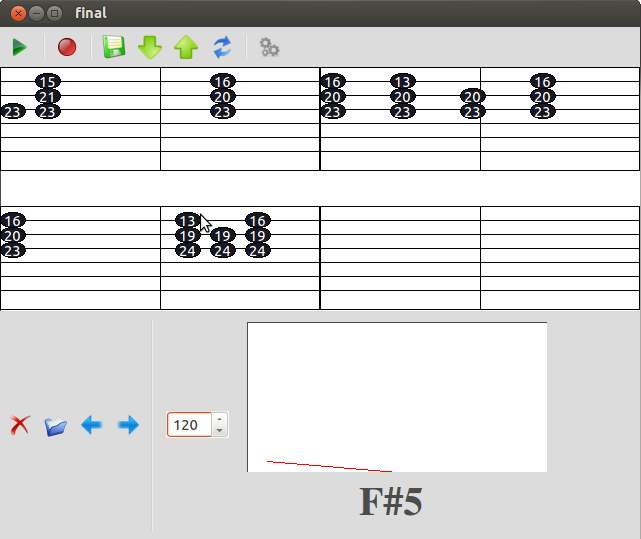
\includegraphics[scale=0.5]{RenduFinal}
\caption{Rendu final de l'application}
\end{figure}

\paragraph{}
Afin de lier l'application cliente et l'application web, nous utilisons un format de sauvegarde partagé par les deux 
langages (C++ et JS), le JSON. Nous avons donc conçu un simple parser JSON afin de pouvoir sauvegarder une partition 
soit sur son PC local, soit dans la base de donnée distante pour la partager avec le monde. Nous avons choisi 
ce format d'enregistrement car il est aisément lisible sur le serveur qui peut alors traiter rapidement les informations 
pour les afficher au utilisateurs, et car c'est un format de plus en plus répandu. Nous aurions pu prendre du XML, mais 
il aurait été moins bien traité côté serveur. De plus, le format JSON consomme moins de place en mémoire que le format XML,
car il est légèrement moins verbeux. L'application possède donc des fonctionnalités de sauvegardes sous forme de fichier et 
de sauvegarde sur le \"cloud\" representé par le site web. Il est possible de réouvrir une partition sauvegardée en local.

\paragraph{}
La bibliothèque FMOD Ex nous permet de récupérer le son entrant de l'application. Elle a été choisi car elle est simple 
d'utilisation tout en étant efficace. Cela nous a permis de nous concentrer sur le traitement de ce son, qui constitue 
une des parties les plus importante du projet. Nous avons suivi l'algorithme du rapport de conception, et y avons apporté 
quelques modifications pour l'implémentation réelle.

\paragraph{}
La bibliothèque Qt ne crée pas de nouveau thread pour sa partie graphique comme Swing par exemple, nous avons donc du créer deux nouveaux 
thread pour l'enregistrement de partitions et l'accordeur. Il a été aisé d'implementer ces thread car Qt nous permet d'en 
faire un héritant d'une de ses classes. Sans ces threads, l'applications serait par exemple bloquée si l'on appuie sur le 
bouton d'enregistrement, car celui ne serait plus accessible une fois l'enregistrement lancé.

\paragraph{}
La quantité de fréquences a traiter étant importante (8192 tous les pas de temps), nous avons décidé d'utiliser 
le tri rapide pour un maximum de performance. Nous avons due y ajouter une surcouche sauvegardant les places de chaque fréquences 
car FMOD assigne chaque volume de fréquence à sa place dans le tableau. Si nous avions uniquement trié le tableau de fréquences 
en fonction du volume, nous n'aurions plus la possibilité de savoir quelle fréquence a le volume le plus haut. 

\paragraph{}
Nous avons choisi de fournir deux classes sous le design pattern du singleton car cela simplifiait beaucoup le développement, et 
car plusieurs instances de ces deux classes serait inutiles. La classe Notes fournit donc toutes les notes possiblement enregistrable 
dans la musique, et la classe Guitar fournit la possibilité de convertir les notes jouées en frettes pour permettre l'affichage de la 
tablature. Nous nous sommes donc plus concentré sur les tablatures pour guitare et non les partitions en général, 
mais il serait possible de l'adapter pour tous les instrument. Il est également possible de changer l'accordage de la guitare, mais 
uniquement en changeant le code, faute d'un manque de temps pour développer cette fonctionnalité.

\paragraph{}
En ce qui concerne la classe graphique principale NoSkin, on y a implanté les éléments nécessaires à l'interface graphique et on lui a assigné un layout de base, tout en considérant le fait que par la suite on pourrait hériter de cette classe pour permettre des interfaces plus personnalisées.
